\documentclass[10pt,a4paper]{article}

%double si on veut une version prof et une version élève. simple si on veut une seule version.
\newcommand{\buildmode}{simple}

\InputIfFileExists{version.tex}{}{}
% Version (définie par le script)
\providecommand{\version}{eleve}

\usepackage{feuillecorrection}
\usepackage{schemaevolution}

%%%à modifier à chaque fois

\renewcommand{\niveau}{1STMG}
\renewcommand{\chapitre}{Révisions}
\renewcommand{\numchap}{1 à 3}
\renewcommand{\theme}{Travail en distanciel}

\begin{document}

\montitre{Révisions des premiers chapitres -- Correction}

%%%%%%%%%%%%%%%%%%%%%%%%%%%%%%%%%%%%%%%%%%%%%%%%%%%%%%%%%%%%%%%%%%%%%%%%%%%%%
\section{Fonctions, généralités}

\begin{corr}[Calculs de début de cours]{1}
\begin{enumerate}[leftmargin=*]
    \item Calculs :
    \begin{tasks}(3)
        \task \(-2+1=-1\)
        \task \(1-2=-1\)
        \task \(1+(-2)=-1\)
        \task \(-5-3=-8\)
        \task \(-4+(-6)=-10\)
        \task \(7-(-2)=7+2=9\)
    \end{tasks}
    \item Écritures simplifiées :
    \begin{tasks}(2)
        \task \(1\times x=x\)
        \task \(-1\times x=-x\)
        \task \(2\times x\times(3\times x+5)=2x(3x+5)\)
        \task \(-4\times x-2\times(3\times 4+x)=-4x-2(3\times 4+x)\)
    \end{tasks}
    Le symbole \(\times\) entre \(3\) et \(4\) ne peut pas être supprimé : \(34\) désignerait un autre nombre.
    \item Réductions :
    \begin{tasks}(2)
        \task \(2x-3x+5+1=-x+6\)
        \task \(4x-x-7-2=3x-9\)
        \task \(-x+2x+3-3=x\)
        \task \(-2x+x+5-8=-x-3\)
    \end{tasks}
\end{enumerate}
\end{corr}

\begin{corr}[Guidé]{2}
\begin{enumerate}[leftmargin=*]
    \item Les températures ont été relevées de 0 h à 24 h.
    \item À 6 h, il faisait \(-2\)°C ; à 15 h, il faisait \(6\)°C.
    \item La température était de \(0\)°C à 2 h, à 10 h et à 22 h.
    \item La température a augmenté de 6 h à 15 h.
    \item La température minimale est \(-2\)°C, atteinte à 6 h ; la température maximale est \(6\)°C, atteinte à 15 h.
    \item L'ensemble de définition de \(f\) est \([0\ ;\ 24]\). L'image de \(6\) par \(f\) est \(-2\), c'est-à-dire \(f(6)=-2\) ; de même \(f(15)=6\). Les antécédents de \(0\) par \(f\) sont \(2\), \(10\) et \(22\).
    \item Tableaux de signes et de variations :
    \begin{center}
    \begin{tikzpicture}
    \tkzTabInit[lgt=1.1,espcl=1.6]{\(t\) /1, \(f(t)\) /1}{\(0\),\(2\),\(10\),\(22\),\(24\)}
    \tkzTabLine{,+,z,-,z,+,z,-,}
    \end{tikzpicture}

    \medskip

    \begin{tikzpicture}
    \tkzTabInit[lgt=1.1,espcl=1.6]{\(t\) /1, \(f\) /2}{\(0\),\(6\),\(15\),\(24\)}
    \tkzTabVar{+/\(1\),-/\(-2\),+/\(6\),-/\(-1\)}
    \end{tikzpicture}
    \end{center}
    \item La température est positive de 0 h à 2 h et de 10 h à 22 h ; elle est négative de 2 h à 10 h et de 22 h à 24 h.

    La température diminue de 0 h à 6 h, augmente de 6 h à 15 h, puis diminue de 15 h à 24 h. Elle atteint son minimum, \(-2\)°C, à 6 h et son maximum, \(6\)°C, à 15 h.
\end{enumerate}
\end{corr}

\begin{corr}{3}
\begin{enumerate}[leftmargin=*]
    \item \(\mathcal{D}_g=[-3\ ;\ 4]\).
    \item \(g(-1)=2\) ; \(g(1)=-1\) ; \(g(4)=1\).
    \item Le nombre \(2\) a un seul antécédent : \(-1\). Les antécédents de \(0\) sont \(-2\), \(0\) et environ \(3,5\).
    \item Les solutions de \(g(x)=-2\) sont \(-3\) et \(2\).
    \item Tableau de signes :
    \begin{center}
    \begin{tikzpicture}
    \tkzTabInit[lgt=1.1,espcl=1.6]{\(x\) /1, \(g(x)\) /1}{\(-3\),\(-2\),\(0\),{\(3{,}5\)},\(4\)}
    \tkzTabLine{,-,z,+,z,-,z,+,}
    \end{tikzpicture}
    \end{center}
    \item Tableau de variations :
    \begin{center}
    \begin{tikzpicture}
    \tkzTabInit[lgt=1.1,espcl=1.6]{\(x\) /1, \(g\) /2}{\(-3\),\(-1\),\(2\),\(4\)}
    \tkzTabVar{-/\(-2\),+/\(2\),-/\(-2\),+/\(1\)}
    \end{tikzpicture}
    \end{center}
\end{enumerate}
\end{corr}

\begin{corr}{4}
\begin{enumerate}[leftmargin=*]
    \item Par exemple : \(h(2)=2^2-4\times 2+3=4-8+3=-1\).
    \begin{center}
    \renewcommand{\arraystretch}{1.5}
    \setlength{\tabcolsep}{0.3cm}
    \begin{tabular}{|c|c|c|c|c|c|c|}
        \hline
        \(x\) & \(0\) & \(1\) & \(2\) & \(3\) & \(4\) & \(5\) \\
        \hline
        \(h(x)\) & \(3\) & \(0\) & \(-1\) & \(0\) & \(3\) & \(8\) \\
        \hline
    \end{tabular}
    \end{center}
    \item Courbe représentative de \(h\) :
    \begin{center}
    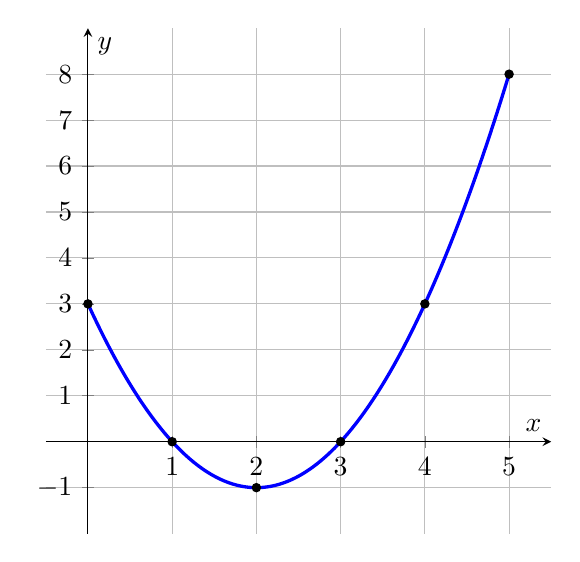
\begin{tikzpicture}
    \begin{axis}[
        axis lines=middle,
        xmin=-0.5, xmax=5.5,
        ymin=-2, ymax=9,
        grid=major,
        xtick={0,1,...,5},
        ytick={-1,0,...,8},
        xlabel={\(x\)},
        ylabel={\(y\)},
        width=8cm,
        height=8cm
    ]
    \addplot[blue, very thick, domain=0:5, samples=100] {x^2-4*x+3};
    \addplot[only marks, mark=*, mark size=1.5pt] coordinates {(0,3)(1,0)(2,-1)(3,0)(4,3)(5,8)};
    \end{axis}
    \end{tikzpicture}
    \end{center}
    \item Les solutions de \(h(x)=0\) sont \(1\) et \(3\).
    \item Tableaux de signes et de variations :
    \begin{center}
    \begin{tikzpicture}
    \tkzTabInit[lgt=1.1,espcl=1.6]{\(x\) /1, \(h(x)\) /1}{\(0\),\(1\),\(3\),\(5\)}
    \tkzTabLine{,+,z,-,z,+,}
    \end{tikzpicture}
    \qquad
    \begin{tikzpicture}
    \tkzTabInit[lgt=1.1,espcl=1.6]{\(x\) /1, \(h\) /2}{\(0\),\(2\),\(5\)}
    \tkzTabVar{+/\(3\),-/\(-1\),+/\(8\)}
    \end{tikzpicture}
    \end{center}
\end{enumerate}
\end{corr}

\begin{corr}{5}
\begin{enumerate}[leftmargin=*]
    \item La fonction \(k\) est décroissante sur \([-4\ ;\ -1]\), croissante sur \([-1\ ;\ 3]\), puis décroissante sur \([3\ ;\ 6]\).

    Le minimum de \(k\) sur \([-4\ ;\ 6]\) est \(-3\), atteint en \(x=-1\). Le maximum de \(k\) sur \([-4\ ;\ 6]\) est \(5\), atteint en \(x=3\).
    \item \(k(x)\) est positif pour \(x\) dans \([-4\ ;\ -3]\) et dans \([1\ ;\ 6]\). \(k(x)\) est négatif pour \(x\) dans \([-3\ ;\ 1]\).
    \item L'équation \(k(x)=0\) a deux solutions : \(-3\) et \(1\).
    \item Une courbe possible :
    \begin{center}
    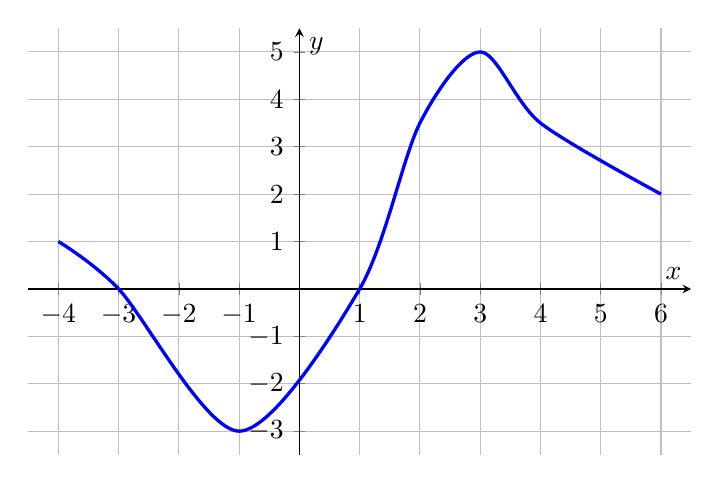
\begin{tikzpicture}
    \begin{axis}[
        axis lines=middle,
        xmin=-4.5, xmax=6.5,
        ymin=-3.5, ymax=5.5,
        grid=major,
        xtick={-4,-3,...,6},
        ytick={-3,-2,...,5},
        xlabel={\(x\)},
        ylabel={\(y\)},
        width=10cm,
        height=7cm
    ]
    \addplot[blue, very thick, smooth] coordinates {(-4,1)(-3,0)(-1,-3)(1,0)(2,3.5)(3,5)(4,3.5)(6,2)};
    \end{axis}
    \end{tikzpicture}
    \end{center}
\end{enumerate}
\end{corr}

\begin{corr}{6}
\begin{enumerate}[leftmargin=*]
    \item Plusieurs courbes sont possibles : elles doivent passer par les points \((-2\ ;\ 3)\), \((1\ ;\ -1)\) et \((4\ ;\ 2)\), descendre sur \([-2\ ;\ 1]\) et monter sur \([1\ ;\ 4]\).
    \item Sur \([-2\ ;\ 1]\), \(m\) est décroissante et passe de \(3\) (positif) à \(-1\) (négatif) : la courbe coupe une seule fois l'axe des abscisses. Sur \([1\ ;\ 4]\), \(m\) est croissante et passe de \(-1\) à \(2\) : la courbe coupe une seule fois l'axe des abscisses. L'équation \(m(x)=0\) a donc exactement deux solutions.
    \item Non, on ne connaît pas leurs valeurs exactes : on sait seulement que l'une, notée \(a\), est dans \(]-2\ ;\ 1[\) et l'autre, notée \(b\), dans \(]1\ ;\ 4[\). On peut tout de même donner l'allure du tableau de signes :
    \begin{center}
    \begin{tikzpicture}
    \tkzTabInit[lgt=1.1,espcl=1.6]{\(x\) /1, \(m(x)\) /1}{\(-2\),\(a\),\(b\),\(4\)}
    \tkzTabLine{,+,z,-,z,+,}
    \end{tikzpicture}
    \end{center}
\end{enumerate}
\end{corr}

%%%%%%%%%%%%%%%%%%%%%%%%%%%%%%%%%%%%%%%%%%%%%%%%%%%%%%%%%%%%%%%%%%%%%%%%%%%%%
\section{Proportions, pourcentages et tableaux croisés}

\begin{corr}[Calculs de début de cours]{7}
\begin{tasks}(3)
    \task \(\dfrac{2}{4}+\dfrac{1}{4}=\dfrac{3}{4}\)
    \task \(\dfrac{4}{6}+\dfrac{1}{6}=\dfrac{5}{6}\)
    \task \(\dfrac{6}{10}-\dfrac{1}{10}=\dfrac{5}{10}=\dfrac{1}{2}\)
    \task \(\dfrac{5}{5}-\dfrac{2}{5}=\dfrac{3}{5}\)
    \task \(\dfrac{2\times 3}{3\times 4}=\dfrac{6}{12}=\dfrac{1}{2}\)
    \task \(\dfrac{5\times 2}{15}=\dfrac{10}{15}=\dfrac{2}{3}\)
\end{tasks}
\end{corr}

\begin{corr}[Guidé]{8}
\begin{enumerate}[leftmargin=*]
    \item Par exemple, à pied en seconde : \(140-80-20=40\).
    \begin{center}
    \renewcommand{\arraystretch}{1.5}
    \begin{tabular}{|l|c|c|c|c|}
        \hline
        & \textbf{Transports en commun} & \textbf{Vélo} & \textbf{À pied} & \textbf{Total} \\
        \hline
        \textbf{Seconde} & \(80\) & \(20\) & \(40\) & \(140\) \\
        \hline
        \textbf{Première} & \(70\) & \(15\) & \(45\) & \(130\) \\
        \hline
        \textbf{Terminale} & \(75\) & \(25\) & \(30\) & \(130\) \\
        \hline
        \textbf{Total} & \(225\) & \(60\) & \(115\) & \(400\) \\
        \hline
    \end{tabular}
    \end{center}
    Vérification : \(225+60+115=400\).
    \item \(\dfrac{140}{400}=0,35\). C'est une fréquence marginale.
    \item \(\dfrac{60}{400}=0,15\).
    \item \(\dfrac{30}{400}=0,075\).
    \item \(\dfrac{45}{130}\approx 0,346\). C'est une fréquence conditionnelle : on se place parmi les élèves de première.
    \item \(\dfrac{20}{60}\approx 0,333\).
\end{enumerate}
\end{corr}

\begin{corr}{9}
\begin{enumerate}[leftmargin=*]
    \item \(n=0,15\times 1\,200=180\) : il y a \(180\) élèves en série STMG.
    \item \(N=\dfrac{84}{0,35}=240\) : l'entreprise compte \(240\) salariés.
    \item \(0,4\times 35=14\) filles, donc \(35-14=21\) garçons.
\end{enumerate}
\end{corr}

\begin{corr}{10}
\begin{enumerate}[leftmargin=*]
    \item \begin{enumerate}
        \item \(\dfrac{150}{500}=0,3\) : fréquence marginale.
        \item \(\dfrac{80}{150}\approx 0,533\) : fréquence conditionnelle.
        \item \(\dfrac{90}{100}=0,9\) : fréquence conditionnelle.
        \item \(\dfrac{150}{500}=0,3\) : fréquence marginale.
    \end{enumerate}
    \item \(\dfrac{60}{500}=0,12\).
    \item Vrai. Parmi les moins de 30 ans : \(\dfrac{80}{150}\approx 0,533\), soit environ \(53\,\%\) paient par téléphone. Parmi les 30 ans et plus : \(\dfrac{70}{350}=0,2\), soit \(20\,\%\). Les effectifs (\(80\) et \(70\)) sont proches, mais les fréquences conditionnelles sont très différentes.
\end{enumerate}
\end{corr}

\begin{corr}[QCM]{11}
\begin{enumerate}[leftmargin=*]
    \item Réponse c) : \(\dfrac{3}{8}=3\div 8=0,375=37,5\,\%\).
    \item Réponse b) : \(0,35\times 800=280\).
    \item Réponse c) : \(\dfrac{45}{0,3}=150\).
    \item Réponse c) : on se place parmi les \(250\) clients qui paient par carte, dont \(60\) ont moins de 30 ans.
\end{enumerate}
\end{corr}

%%%%%%%%%%%%%%%%%%%%%%%%%%%%%%%%%%%%%%%%%%%%%%%%%%%%%%%%%%%%%%%%%%%%%%%%%%%%%
\section{Évolutions}

\begin{corr}[Calculs de début de cours]{12}
\begin{enumerate}[leftmargin=*]
    \item Solutions :
    \begin{tasks}(4)
        \task \(2x=8\), \(x=4\)
        \task \(5x=-15\), \(x=-3\)
        \task \(x=6\div 0,5=12\)
        \task \(x=3-1,2=1,8\)
    \end{tasks}
    \item Fractions :
    \begin{tasks}(6)
        \task \(\dfrac{11}{10}\)
        \task \(\dfrac{9}{10}\)
        \task \(\dfrac{5}{4}\)
        \task \(\dfrac{3}{4}\)
        \task \(\dfrac{3}{2}\)
        \task \(\dfrac{4}{5}\)
    \end{tasks}
    \item \(1,1\times 1,2=\dfrac{11}{10}\times\dfrac{12}{10}=\dfrac{132}{100}=1,32\).
\end{enumerate}
\end{corr}

\begin{corr}[Guidé]{13}
\begin{enumerate}[leftmargin=*]
    \item Schéma complété :
    \schemaevolution{60}{45}{-25\,\%}{\times 0,75}
    \item Une baisse de \(25\,\%\) correspond à \(t=-0,25\), donc \(CM=1+(-0,25)=0,75\).
    \item \(V_F=60\times 0,75=45\) : le prix soldé est \(45\) \euro.
    \item \(t=\dfrac{54-45}{45}=\dfrac{9}{45}=0,2\) : le prix a augmenté de \(20\,\%\).
    \item Non, \(54\neq 60\). \(CM_{\text{global}}=0,75\times 1,2=0,9\), donc \(t_{\text{global}}=0,9-1=-0,1\) : sur l'ensemble des deux évolutions, le prix a baissé de \(10\,\%\). On vérifie : \(60\times 0,9=54\).
\end{enumerate}
\end{corr}

\begin{corr}{14}
\begin{center}
\renewcommand{\arraystretch}{1.5}
\begin{tabular}{|C{0.18\textwidth}|C{0.18\textwidth}|C{0.18\textwidth}|C{0.18\textwidth}|}
    \hline
    \textbf{Valeur initiale} & \textbf{Taux d'évolution} & \textbf{Coefficient multiplicateur} & \textbf{Valeur finale} \\ \hline
    \(40\) \euro & \(+15\,\%\) & \(1,15\) & \(46\) \euro \\ \hline
    \(250\) \euro & \(-8\,\%\) & \(0,92\) & \(230\) \euro \\ \hline
    \(120\) \euro & \(+5\,\%\) & \(1,05\) & \(126\) \euro \\ \hline
    \(80\) \euro & \(-25\,\%\) & \(0,75\) & \(60\) \euro \\ \hline
    \(60\) \euro & \(-40\,\%\) & \(0,6\) & \(36\) \euro \\ \hline
\end{tabular}
\end{center}
Ligne 4 : \(CM=\dfrac{60}{80}=0,75\). Ligne 5 : \(V_I=\dfrac{36}{0,6}=60\).
\end{corr}

\begin{corr}{15}
\begin{enumerate}[leftmargin=*]
    \item Dans chaque schéma, le coefficient global est le produit des deux coefficients.

    \schemaDeuxevolutions{500}{600}{540}{+20\,\%}{1,2}{-10\,\%}{0,9}{\times 1,08}{+8\,\%}

    \schemaDeuxevolutions{80}{60}{75}{-25\,\%}{0,75}{+25\,\%}{1,25}{\times 0,9375}{-6,25\,\%}
    \item Non : \(0,75\times 1,25=0,9375<1\). Après une baisse de \(25\,\%\) puis une hausse de \(25\,\%\), on obtient une baisse globale de \(6,25\,\%\).
    \item \(CM_{\text{global}}=1,03\times 1,02=1,0506\), donc le loyer a augmenté de \(5,06\,\%\) sur les deux années.
\end{enumerate}
\end{corr}

\begin{corr}[Vrai ou faux]{16}
\begin{enumerate}[leftmargin=*]
    \item Faux : \(1,1\times 1,1=1,21\), c'est une hausse de \(21\,\%\).
    \item Vrai : \(0,5\times 2=1\).
    \item Vrai : \(1,3\times 0,7=0,91\), c'est une baisse de \(9\,\%\).
    \item Faux : on cherche \(CM\) tel que \(0,8\times CM=1\), soit \(CM=\dfrac{1}{0,8}=1,25\). Il faut une hausse de \(25\,\%\).
\end{enumerate}
\end{corr}

%%%%%%%%%%%%%%%%%%%%%%%%%%%%%%%%%%%%%%%%%%%%%%%%%%%%%%%%%%%%%%%%%%%%%%%%%%%%%
\section{Problèmes}

\begin{corr}[Ventes de vélos]{17}
\begin{enumerate}[leftmargin=*]
    \item \(\dfrac{250}{700}\approx 0,357\).
    \item \(\dfrac{120}{300}=0,4\).
    \item Vélos électriques : \(300\times 1,15=345\). Vélos classiques : \(400\times 0,9=360\).
    \item Total en 2026 : \(345+360=705\). \(t=\dfrac{705-700}{700}\approx 0,007\), soit une hausse d'environ \(0,7\,\%\).
    \item Les deux taux ne s'appliquent pas aux mêmes quantités (\(300\) vélos électriques et \(400\) vélos classiques) : on ne peut pas les additionner. La hausse porte sur \(45\) vélos et la baisse sur \(40\) vélos, d'où une hausse totale de seulement \(5\) vélos, soit environ \(0,7\,\%\).
\end{enumerate}
\end{corr}

\begin{corr}[Population d'une commune]{18}
\begin{enumerate}[leftmargin=*]
    \item \(\mathcal{D}_p=[1990\ ;\ 2025]\). \(p(2000)=84\) et \(p(2020)=108\) : la commune comptait \(84\,000\) habitants en 2000 et \(108\,000\) en 2020.
    \item \(t=\dfrac{108-84}{84}=\dfrac{24}{84}\approx 0,286\), soit une hausse d'environ \(28,6\,\%\).
    \item La population a atteint \(100\,000\) habitants vers 2014. L'antécédent de \(100\) par \(p\) est environ \(2014\).
    \item Tableau de variations :
    \begin{center}
    \begin{tikzpicture}
    \tkzTabInit[lgt=1.1,espcl=2]{\(t\) /1, \(p\) /2}{\(1990\),\(2025\)}
    \tkzTabVar{-/\(80\),+/\(112\)}
    \end{tikzpicture}
    \end{center}
    La population de la commune a augmenté de 1990 à 2025, passant de \(80\,000\) à \(112\,000\) habitants.
    \item \(112\times 1,02\times 1,02=112\times 1,0404\approx 116,5\) : on prévoit environ \(116\,500\) habitants en 2027.
\end{enumerate}
\end{corr}

\end{document}
